\chapter{Affine Approximation of the Non-Linear Model}
\label{ch:affine}
\thispagestyle{empty}
\newcommand*{\vertbar}{\rule[-1ex]{0.5pt}{2.5ex}}
\newcommand*{\horzbar}{\rule[.5ex]{2.5ex}{0.5pt}}
The forward map, introduced in Chapter~\ref{ch:formodel}, poses a weakly non-linear forward problem.
One could tackle the non-linearity by treating the inverse problem as a linear inverse problem and then iteratively updating the non-linear part after each parameter sample.
Instead, as in Fig.~\ref{fig:affinStrat} illustrated, we approximate the non-linear model using an affine map, which is a linear map with a translation, e.g. $\bm{A}\bm{x} + \bm{b}$, and maps Gaussians onto Gaussians.
Here we find an affine map $\bm{M}$ based on the linear model $\bm{A}_L$ that provides an approximation of the non-linear model $\bm{A}(\bm{x})$ for parameters $\bm{x}$ near the posterior mean $\bm{\mu}_{\bm{x}|\bm{y}}$.
\begin{figure}[htb!]
	\centering
	\begin{tikzpicture}
		\node[rectnode] at (0,0) (Oy)    {$\bm{y}$};
		\node[roundnode2] at (0,-2) (x)     {$\bm{x}$};
		\node[roundnode2] at (1.75,-4) (V)    {$\bm{V}$};%{$\bm{A}_{NL}\bm{x}$};
		\node[roundnode2] at (-1.75,-4) (W)    {$\bm{W}$};%{$\bm{A}_L\bm{x}$};
		\draw[->, very thick] (Oy.south) -- (x.north); 
		\draw[->, very thick] (x) -- (V); 
		\draw[->, very thick] (x) -- (W); 
		\draw[->, very thick] (W.east) --  (V.west); 
		\node[align=center] at (1,0) (l1) {data};
		\node[align=center] at (3.5,-2) (f2) {ozone profiles from $\pi(\bm{x}|\bm{y}) $};
		\node[align=center] at (1.75,-1) (l1) {$\pi(\lambda , \gamma  | \bm{y})$ with $\bm{A}_L$};
		
		
		\node[align=center] at (-4.25,-4) (f3) {linear forward model};
		\node[align=center] at (4.75,-4) (f4) {non-linear forward model};
		\node[align=center] at (0,-5) (f5) {$\bm{A}(\bm{x}) \approx \bm{M A}_L \bm{x}$ };
		
		\node[align=center] at (0,-4) (f5) {affine map \\ $\bm{M}$};
		
	\end{tikzpicture}
	\caption[Strategy to find affine map.]{The strategy to find the affine map consists of first evaluating the marginal posterior for ozone $\pi(\lambda , \gamma  | \bm{y})$ based on the linear forward model. Based on ozone samples from the full posterior, we find an affine map $\bm{M}$ which approximates between noise-free linear data $\bm{A}_L$ and noise-free non-linear data $\bm{A}(\bm{x})$.}
	\label{fig:affinStrat}
\end{figure}

\section{Finding an Affine Map}

We find an affine map by creating the vector spaces $\bm{W}$ based on the linear forward model and $\bm{V}$ based on the non-linear forward model with ground truth pressure and temperature.
More specifically $m-1$ samples $\bm{x}^{(j)} \sim \pi(\bm{x}|\bm{y})$, for $j = 2, \dots,m$, from the posterior and the posterior mean $\bm{\mu}_{\bm{x}|\bm{y}}$ generate,
\begin{align*}
	\bm{W} = \begin{bmatrix}
		\vert& \vert&   &  \vert & & \vert \\
		\bm{A}_{L}  \bm{\mu}_{\bm{x}|\bm{y}} & \bm{A}_{L}  \bm{x}^{(2)}   &  \cdots& \bm{A}_{L} \bm{x}^{(j)} &  \cdots & \bm{A}_{L} \bm{x}^{(m)} \\
		\vert& \vert&   &  \vert & & \vert 
	\end{bmatrix}
	\in \mathbb{R}^{m \times m}
\end{align*}\noindent and
\begin{align*}
	\bm{V} = \begin{bmatrix}
		\vert& \vert&   &  \vert & & \vert \\
		\bm{A}(\bm{\mu}_{\bm{x}|\bm{y}} ) & \bm{A}(\bm{x}^{(2)}) &  \cdots& \bm{A}(\bm{x}^{(j)}) &  \cdots & \bm{A} (\bm{x}^{(m)})  \\
		\vert&\vert&   &  \vert & & \vert 
	\end{bmatrix} = 
	\begin{bmatrix}
		\begin{array}{ccc}
			\horzbar & v_{1} & \horzbar \\
			& \vdots    &          \\
			\horzbar & v_{j} & \horzbar \\
			& \vdots    &          \\
			\horzbar &v_{m} & \horzbar
		\end{array}
	\end{bmatrix}\in \mathbb{R}^{m \times m} \, .
\end{align*}
Then the non-linear forward model is approximated as 
\begin{align}
	\bm{A}(\bm{x}) \approx \bm{M A}_L \bm{x} \, , \label{eq:AffineM}
\end{align}
where we solve $v_j =r_j \bm{W}$ for each row $r_j$ in
\begin{align*}
	\bm{V}\bm{W}^{-1} = \bm{M} =
	\begin{bmatrix}
		\begin{array}{ccc}
			\horzbar & r_{1} & \horzbar \\
			& \vdots    &          \\
			\horzbar & r_{j} & \horzbar \\
			& \vdots    &          \\
			\horzbar &r_{m} & \horzbar
		\end{array}
	\end{bmatrix}\, \in \mathbb{R}^{m \times m} .
\end{align*}
using the Python function \texttt{numpy.linalg.solve}.
This is feasible since every noise-free measurement is independent of each other, and then every row $v_j$ of $\bm{V} \in \mathbb{R}^{m \times m}$ is independent of each other as well.
For an $\bm{x} = \bm{\mu}_{\bm{x}|\bm{y}} + \Delta \bm{x}$ we rewrite Eq.~\ref{eq:AffineM} to
\begin{align}
	\bm{A}(\bm{x})  \approx \underbrace{  \bm{M A}_L  \bm{\mu}_{\bm{x}|\bm{y}} }_{= \bm{A}( \bm{\mu}_{\bm{x}|\bm{y}} )  }+  \underbrace{\bm{M A}_L  \Delta \bm{x} }_{= \bm{A}^{\prime}( \bm{\mu}_{\bm{x}|\bm{y}} )  \Delta \bm{x} }\, \\
	=    \underbrace{ \bm{A}^{\prime}( \bm{\mu}_{\bm{x}|\bm{y}} ) \bm{x}}_{ \bm{A}\bm{x}}  +  \underbrace{ \bm{A}( \bm{\mu}_{\bm{x}|\bm{y}} )  - \bm{A}^{\prime}( \bm{\mu}_{\bm{x}|\bm{y}} ) \bm{\mu}_{\bm{x}|\bm{y}}}_{  \bm{b}}
\end{align}
to show that $ \bm{M}:\bm{A}_L\bm{x} \rightarrow \bm{A}(\bm{x})$ is an affine map.







%	\centering
%	\begin{tikzpicture}
%		\node[rectnode] at (2,-4) (NL)    {$\bm{V}$};
%		\node[rectnode] at (-2,-4) (L)    {$\bm{W}$};
%		\draw[<-, very thick] (NL.west) -- (L.east); 
%		\node[align=center] at (-5.5,-4) (f3) {linear forward model};
%		\node[align=center] at (5.5,-4) (f4) {non-linear forward model};
%		\node[align=center] at (0,-5) (f5) {$\bm{A}(\bm{x})  \approx \bm{M A}_L  \bm{x} $ };
%		\node[align=center] at (0,-4) (f5) {affine Map \\ $\bm{M}$};
%	\end{tikzpicture}
%	\caption[Schematics of the affine map]{This figure shows the schematic representation of how the affine map $\bm{M}$ approximates the non-linear forward model. Here, $\bm{V}$ contains values produced by the linear forward model, and $\bm{W}$ contains the corresponding values from the non-linear forward model. Both $\bm{V}$ and $\bm{W}$ are affine subspaces over the same field. The affine map $\bm{M}$ projects elements from the linear forward model space $\bm{V}$ onto their counterparts in the non-linear forward model space $\bm{W}$. More specifically, the non-linear noise-free data vector $\bm{A} (\bm{x}) $ is approximated by the affine map and the linear forward model so that  $\bm{A} (\bm{x})  \approx  \bm{M A}_L  \bm{x}$.}
%	\label{fig:AffSchem}
%\end{figure}


%Alternatively, one can also determine this map using other methods, e.g. machine learning methods or matrix inversion, which in our case did not give better results.

The relative RMS difference $\lVert \text{vec}(\bm{M}\bm{W}) - \text{vec}(\bm{V})  \rVert_{L^2} / \lVert \text{vec}(\bm{M}\bm{W}) \rVert_{L^2} $ between the mapped linear noise-free data and the non-linear noise-free data is approximately $0.001\%$.
This is much smaller than the relative RMS difference between $\bm{W}$ and $\bm{V}$ of about $1\%$.
\begin{figure}[t!]
	\centering
	%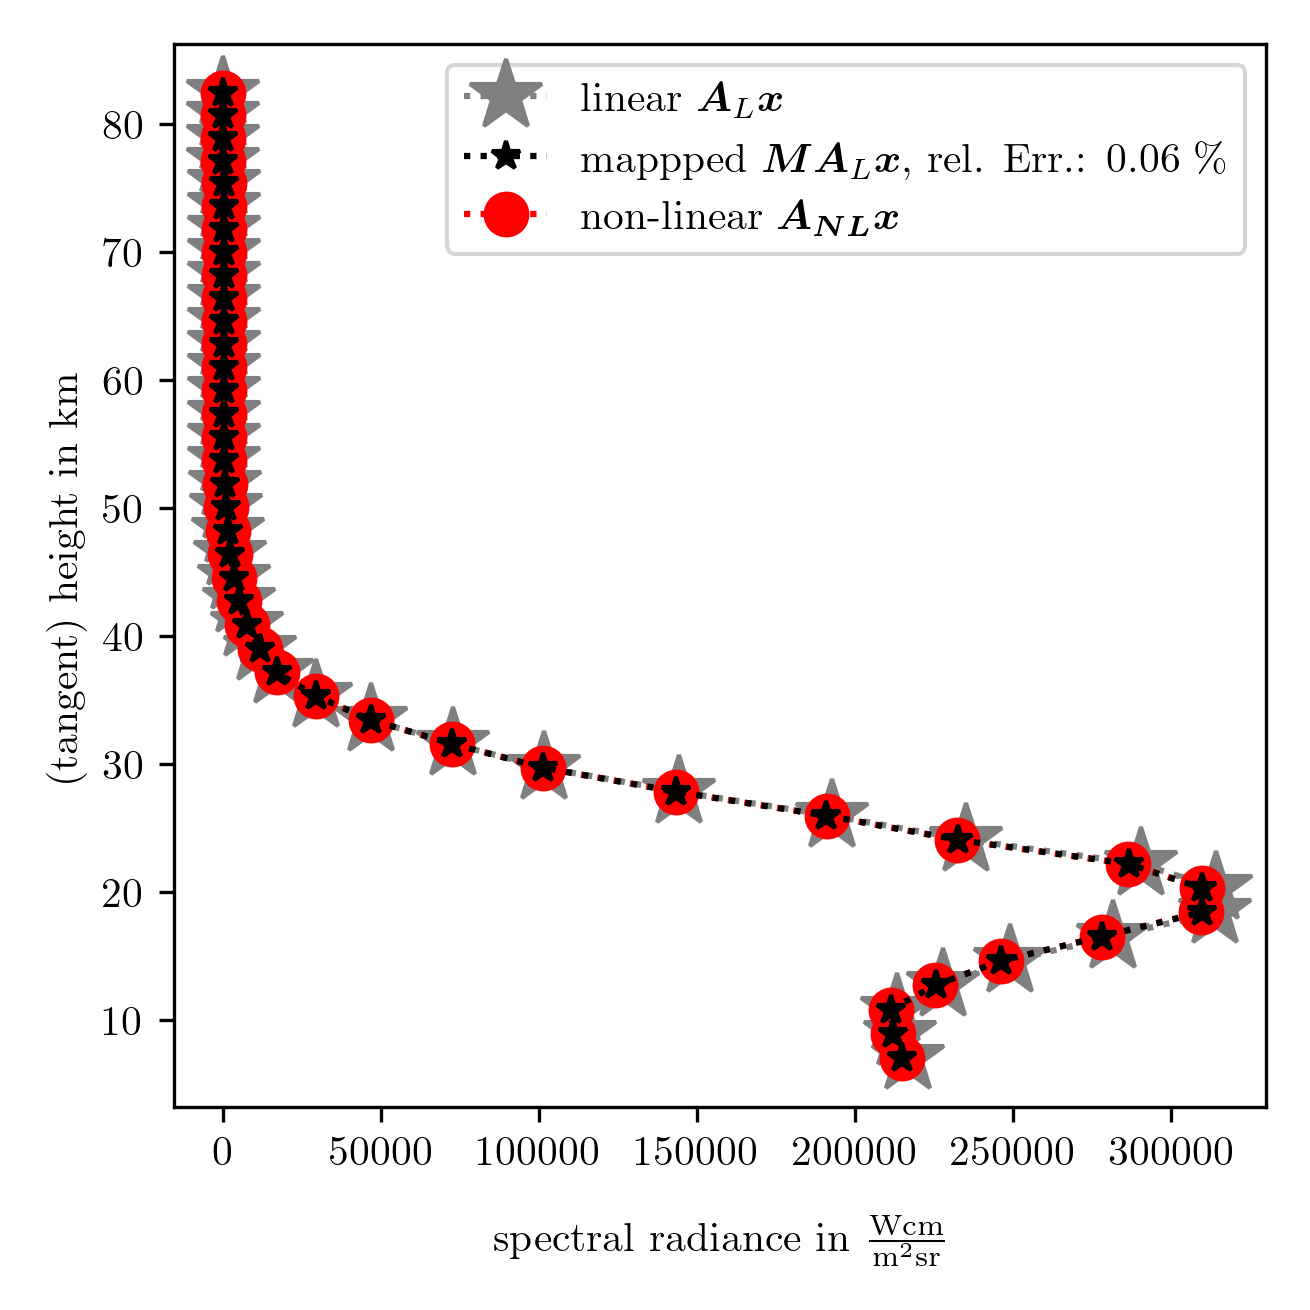
\includegraphics{SampMapAssesment.png}
	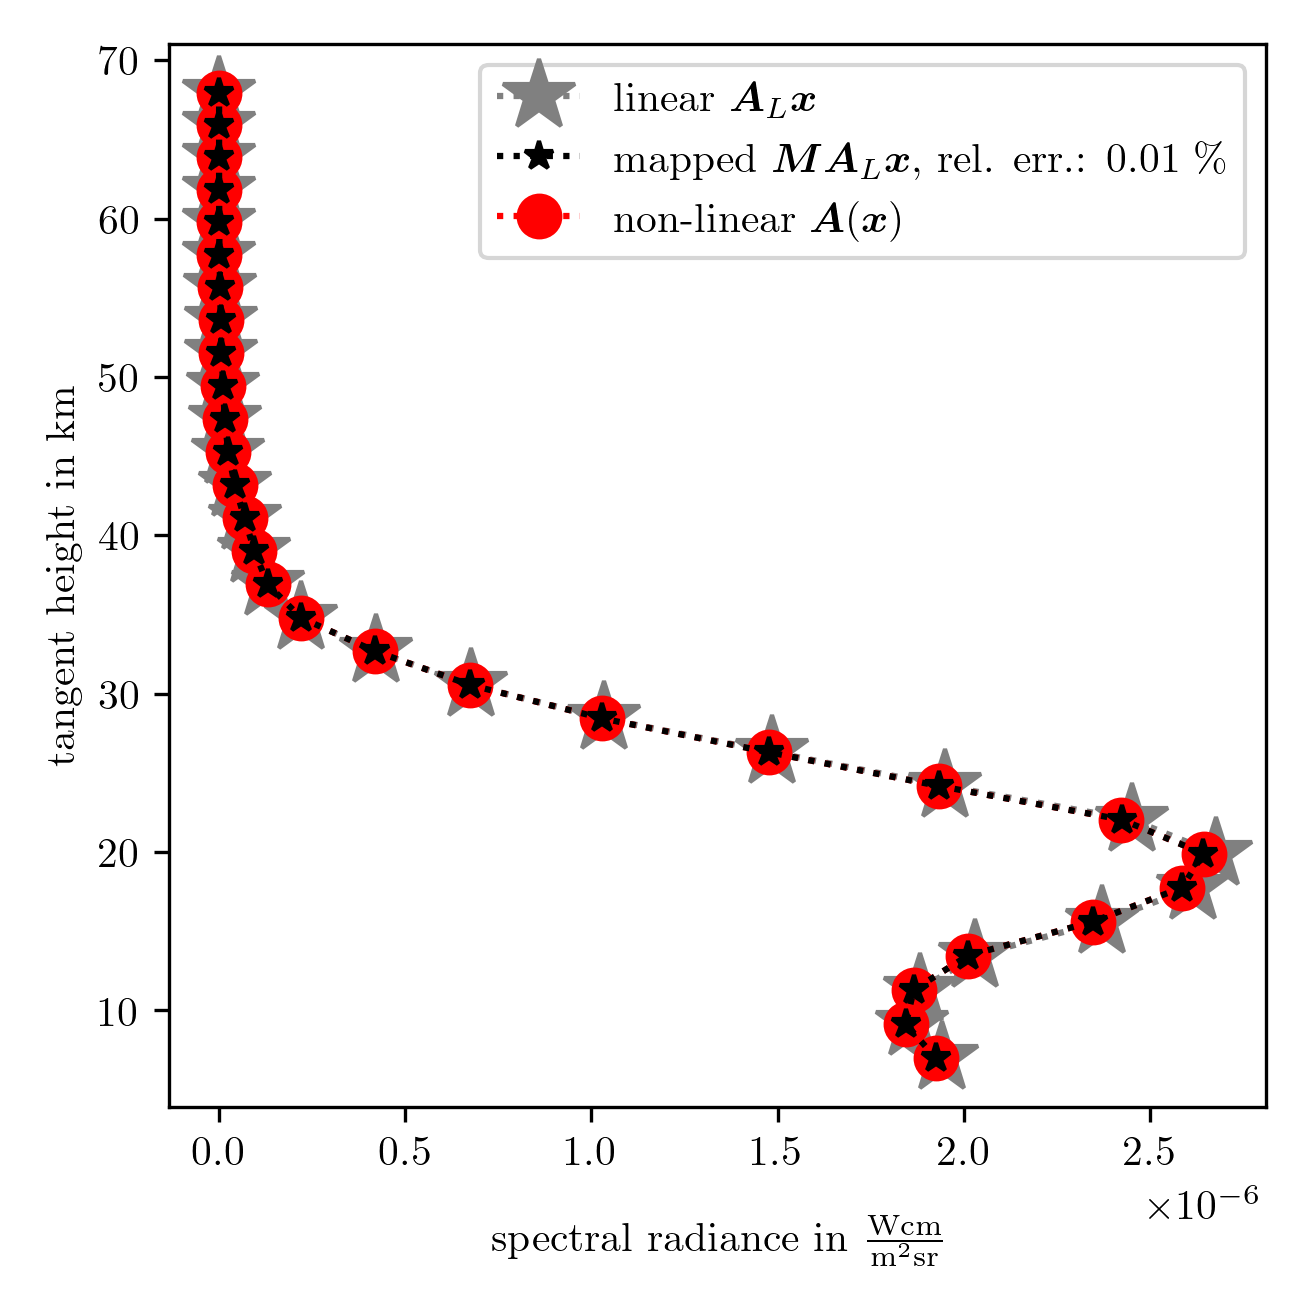
\includegraphics{SampMapAssesmentTT.png}
	\caption[Assessment of affine map.]{Assessment of how well we can approximate noise-free non-linear data $\bm{A}(\bm{x})$  (red circles) with noise-free linear data $\bm{A}_L\bm{x}$ (grey stars) and the previously calculated affine map $\bm{M}$. The approximated noise-free data (black stars) has a relative RMS error of $\approx 0.06\%$ compared to the true non-linear noise-free data.
		The ozone sample to generate this noise-free data has not been used to create the affine map.}
	\label{fig:MapAsses}
\end{figure}
Fig.~\ref{fig:MapAsses} shows the mapping for one posterior ozone sample with a relative RMS error $\approx0.06\%$.
This posterior ozone sample has not been used to create this mapping; in other words, this is an unseen event not occurring in the training data.
Consequently, from here onwards, we use the approximated forward map.
\section{Marginal and then Conditional Posterior -- Ozone}

Again, we use the MTC scheme and the exact same setup and procedure as in Sec. \ref{sec:FirstO3Post} to evaluate the marginal posterior and then the full conditional posterior of ozone with similar computational time.

\begin{figure}[ht!]
	\centering
	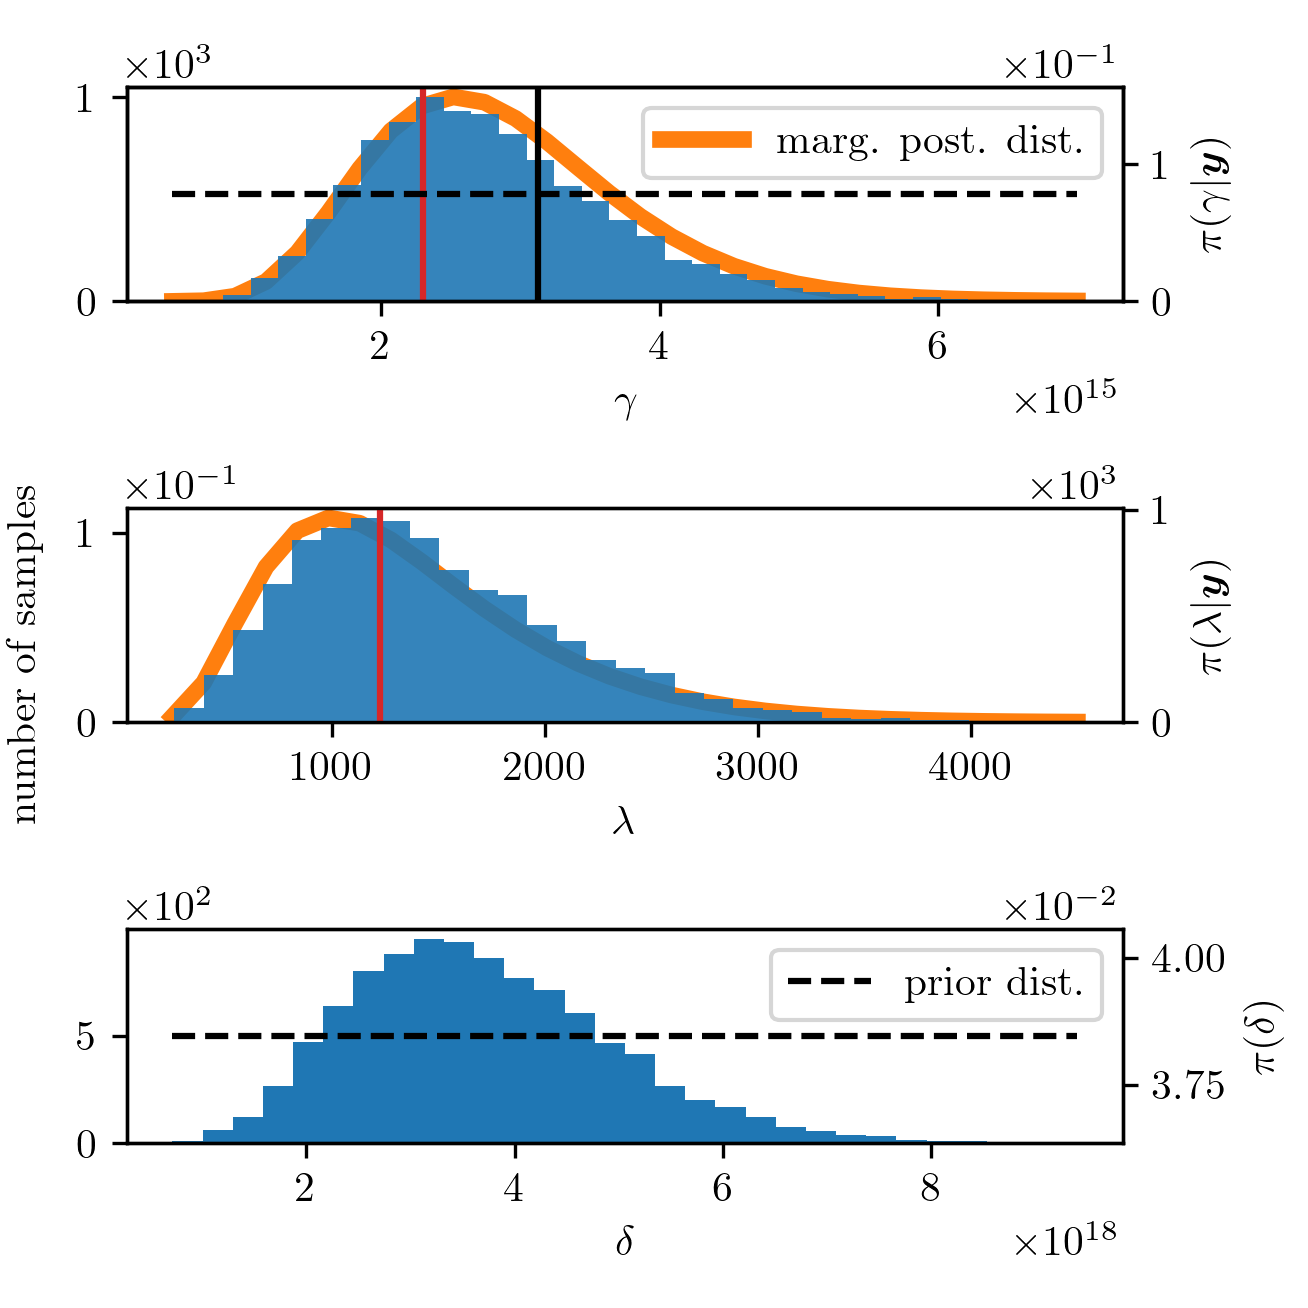
\includegraphics{secMargO3Res.png}
	\caption[Marginal posterior histograms and TT approximation as well as hyper-prior distribution.]{The TT approximation of the marginal posterior in orange and the samples as a histogram, as well as the prior distribution with a dotted line. We sample $\lambda$ and $\gamma$ using the MWG algorithm and then calculate $\delta$ for every sample of the marginal posterior. The regularised parameter corresponding to the best regularised solution (see Fig.~\ref{fig:O3SolplsReg} and Fig.~\ref{fig:LCurve}) is marked with the red vertical line. We mark the ground truth noise precision with the back vertical line.}
	\label{fig:MargPostHistTT}
\end{figure}
The marginal posterior is defined as in Eq.~\ref{eq:MargPostAppl}, but with the approximated forward model.
The MWG is initialised at the mode of $\pi(\lambda,\gamma| \bm{y})$ and $f(\lambda)$ and $g(\lambda)$ are approximated around the mode as in Sec. \ref{subsec:FirstMargPost} (see Eq.~\ref{eq:fAprox} and Eq.~\ref{eq:gAprox}).
We take $N = 10000$ plus $N_{\text{burn-in}} = 100$ steps in $\approx 0.5$s.
The IACTs provided by~\cite{drikHesse} are $\tau_{\text{int}, \gamma} \approx 5.2 \pm 0.3$ and $\tau_{\text{int}, \lambda} = 11 \pm 1 $ (see Fig. \ref{fig:IATCSecO3gam} and Fig.~\ref{fig:IATCSecO3lam}) and similar to the previously calculated values.
We plot the samples in Fig. \ref{fig:MargPostHistTT} as well as the TT approximation of the marginal posterior using 400 function evaluations (same grid; same number of ranks; see Sec.~\ref{subsec:FirstMargPost}).
The relative RMS error of the TT approximation over the whole grid and the relative RMS approximation error of $\pi(\lambda,\gamma| \bm{y})$ due to the approximations of $f(\lambda)$ and $g(\lambda)$ are both $\approx 8 \%$.

\begin{figure}[ht!]
	\centering
	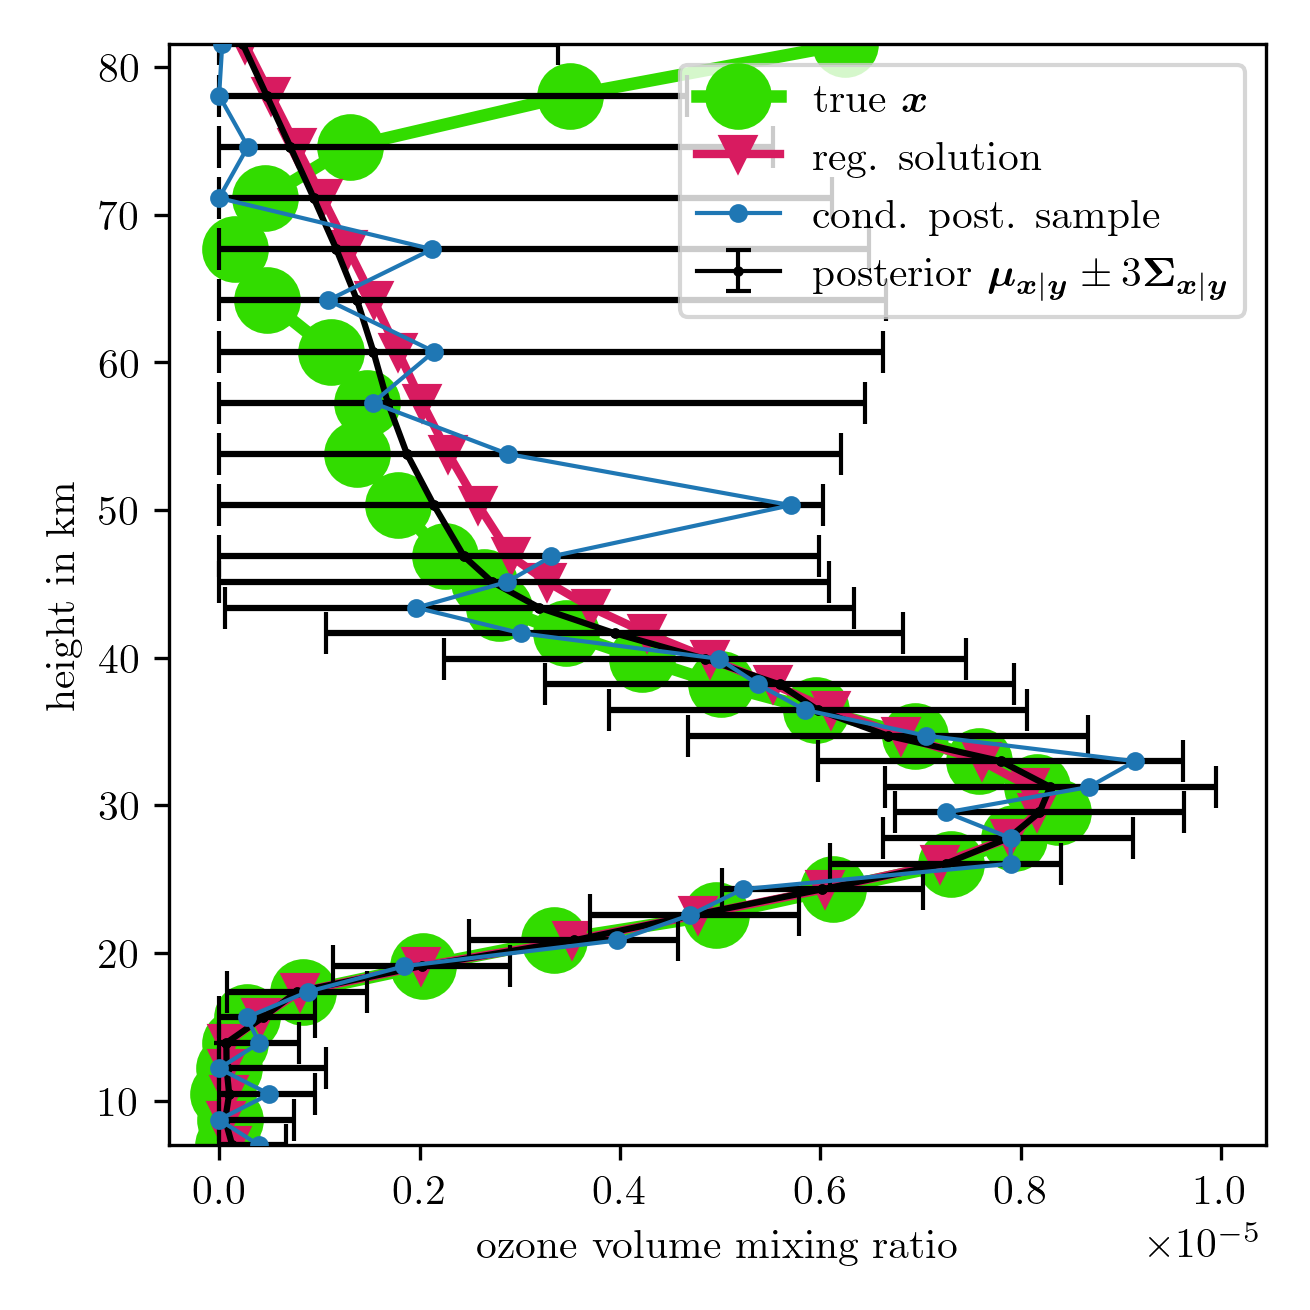
\includegraphics{SecRecResinclRegandSampl.png}
	%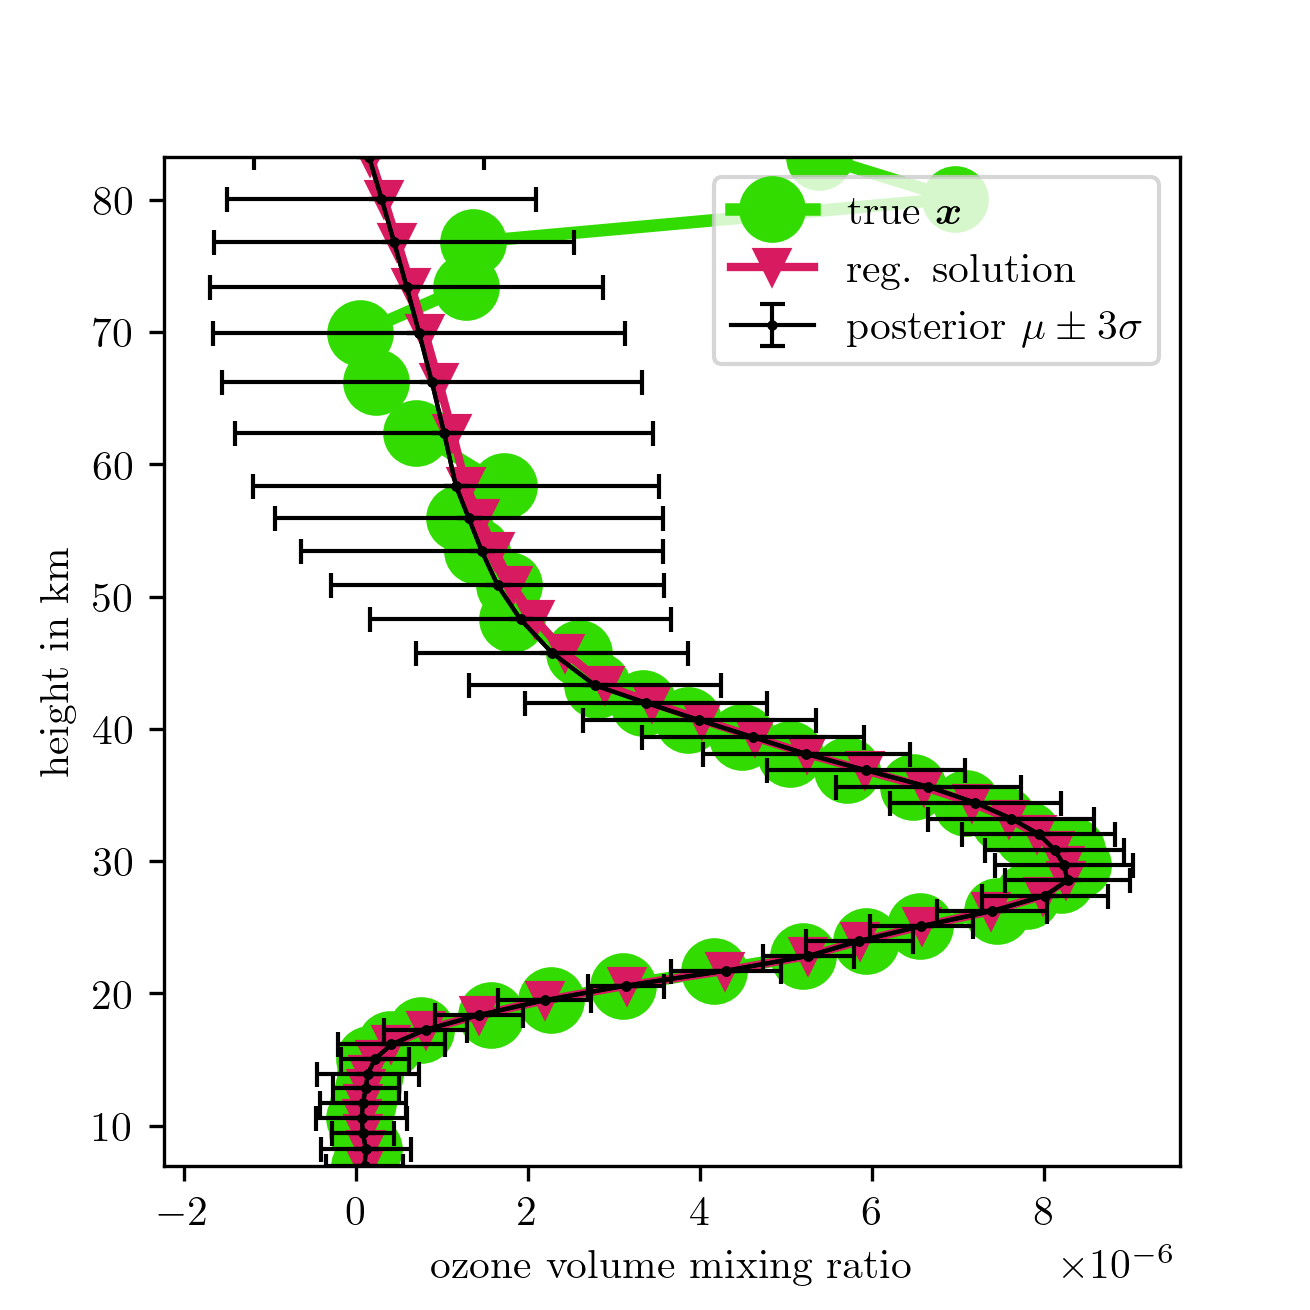
\includegraphics{SecRecResinclReg.png}
	\caption[Full posterior mean and variance of ozone and the regularised solution compared to the ground truth.]{Full posterior mean and variance and one ozone sample from the full posterior. We plot the regularised solution on top of the ground truth ozone profile in green. The results are based on the approximated forward model $\bm{M}\bm{A}_L$.}
	\label{fig:O3SolplsReg}
\end{figure} 
Again, we calculate the full posterior mean $\bm{\mu}_{\bm{x}|\bm{y}}$, see Eq.~\ref{eq:MeanInt}, and covariance matrix $\bm{\Sigma}_{ \bm{x}|\bm{y}}$~\ref{eq:CovInt} as weighted expectation.
We plot the results and one sample of $\pi(\bm{x}|\bm{y})$, which represents a feasible solution to this inverse problem, in Fig.~\ref{fig:O3SolplsReg}, as well as the regularised solution (see next section), and one sample from the posterior.
We can see that the ground truth lies within the STD around the mean, except for the peak at around $80$km.
Compared to the previously calculated mean and variance based on the linear forward model $\bm{A}_L$ (see \ref{fig:O3Samp}), the posterior distribution based on $\bm{M A}_L$ does not differ significantly.
This is expected since the difference between the linear and non-linear forward map of $\approx 1 \%$ is small.
%\clearpage


%Then we are able to define a linear model $ \bm{A} \coloneqq \bm{M} \bm{A}_{L}$, which approximates the non-linear model.
%Here, we give a brief introduction to affine maps.
%
%An affine map is any linear map between two vector spaces or affine spaces, where an affine space does not need to preserve a zero origin (see~\cite[Def. 2.3.1]{berger2009geometry}). \textcolor{red}{no it's not}
%In other words, an affine map does not need to map to the origin of the associated vector space.
%An affine map is a linear map on vector spaces, including a translation, or, in the words of my supervisor, C. F., a Taylor series of first order. \textcolor{red}{it is not a linear map , the origin of the domain to the origin of the range, fix this sentence - -it makes no sense.}
%For more information on affine spaces and maps, we refer to the books~\cite{berger2009geometry, katsumi1994affine}. \textcolor{red}{don't say that, say that it is a linear map plus a constant.}
%
%\textcolor{red}{these are horrible books. No wonder you have a garbled idea and description. All affine maps look like y = Ax+b where A is linear and b is a constant. What's so difficult about that?
%	I asked a LLM:
%	Please give a simple definition of an affine map (between two vector spaces)
%	Sure! A simple definition of an affine map between two vector spaces is:
%	An affine map is a function between vector spaces that preserves straight lines and has the form
%	$>f(x)=Ax+b>$
%	where A is a linear transformation and b is a fixed vector.
%	So it’s like a linear map, but with a shift. }